\documentclass[11pt]{article}

\usepackage[margin=0.78in]{geometry}
\usepackage{fontspec}
\usepackage{microtype}
\usepackage{booktabs}
\usepackage{graphicx}
\usepackage{subcaption}
\usepackage{xcolor}
\usepackage{hyperref}
\usepackage{enumitem}
\usepackage{float}

\setmainfont{Georgia}
\setsansfont{Segoe UI}
\setmonofont{Consolas}

\definecolor{ink}{HTML}{1F2937}
\definecolor{accent}{HTML}{0F766E}
\definecolor{accentlight}{HTML}{E6FFFB}
\definecolor{muted}{HTML}{5B6470}

\hypersetup{
  colorlinks=true,
  linkcolor=accent,
  urlcolor=accent
}

\pagestyle{empty}
\setlength{\parindent}{0pt}
\setlength{\parskip}{0.52em}

\begin{document}
\color{ink}

{\sffamily
\begin{center}
  {\Large\bfseries Appearance-Factored LeWM-lite on Official PushT}\\[0.35em]
  {\large Reliable Rerun and Ablation Summary}\\[0.45em]
  {\small April 26, 2026}
\end{center}
}

\vspace{0.2em}
\fcolorbox{accent}{accentlight}{%
  \parbox{\dimexpr\linewidth-2\fboxsep-2\fboxrule\relax}{
    \textbf{Bottom line.} The Stage 2 reliability check favors \textbf{Baseline LeWM}: \textbf{25/400} successes at epoch 50, versus \textbf{22/400} for \textbf{v1\_current} and \textbf{20/400} for \textbf{v2\_app\_nuisance\_only}. Stage 1 produced useful Appearance-Factored leads, but those leads did not persist after the longer two-seed check.
  }
}

\section*{Architecture and Design Principle}
Appearance-Factored LeWM-lite (AF-LeWM-lite) keeps the LeWM planning contract intact. Here, AF means appearance-factored: the added branch factors appearance information into \texttt{app\_emb}, while planning still uses the dynamics latent \texttt{emb}. The action block encoder is inherited from baseline LeWM.

Pixels are encoded by a shared ViT-tiny backbone; the dynamics projection head produces \texttt{emb}, action blocks are encoded separately, and the autoregressive predictor rolls the dynamics latent forward under candidate actions. Planning uses terminal latent distance between predicted dynamics and the goal dynamics latent.

The AF extension adds an appearance projection head \texttt{app\_emb} used only for representation shaping during training. v1 adds dynamics invariance under appearance augmentation and a cross-covariance penalty between \texttt{emb} and \texttt{app\_emb}. v2 adds sequence-consistent augmentation parameters, stop-gradient invariance, an appearance nuisance head, and a gradient-reversal nuisance head on the dynamics branch.

\begin{figure}[H]
\centering
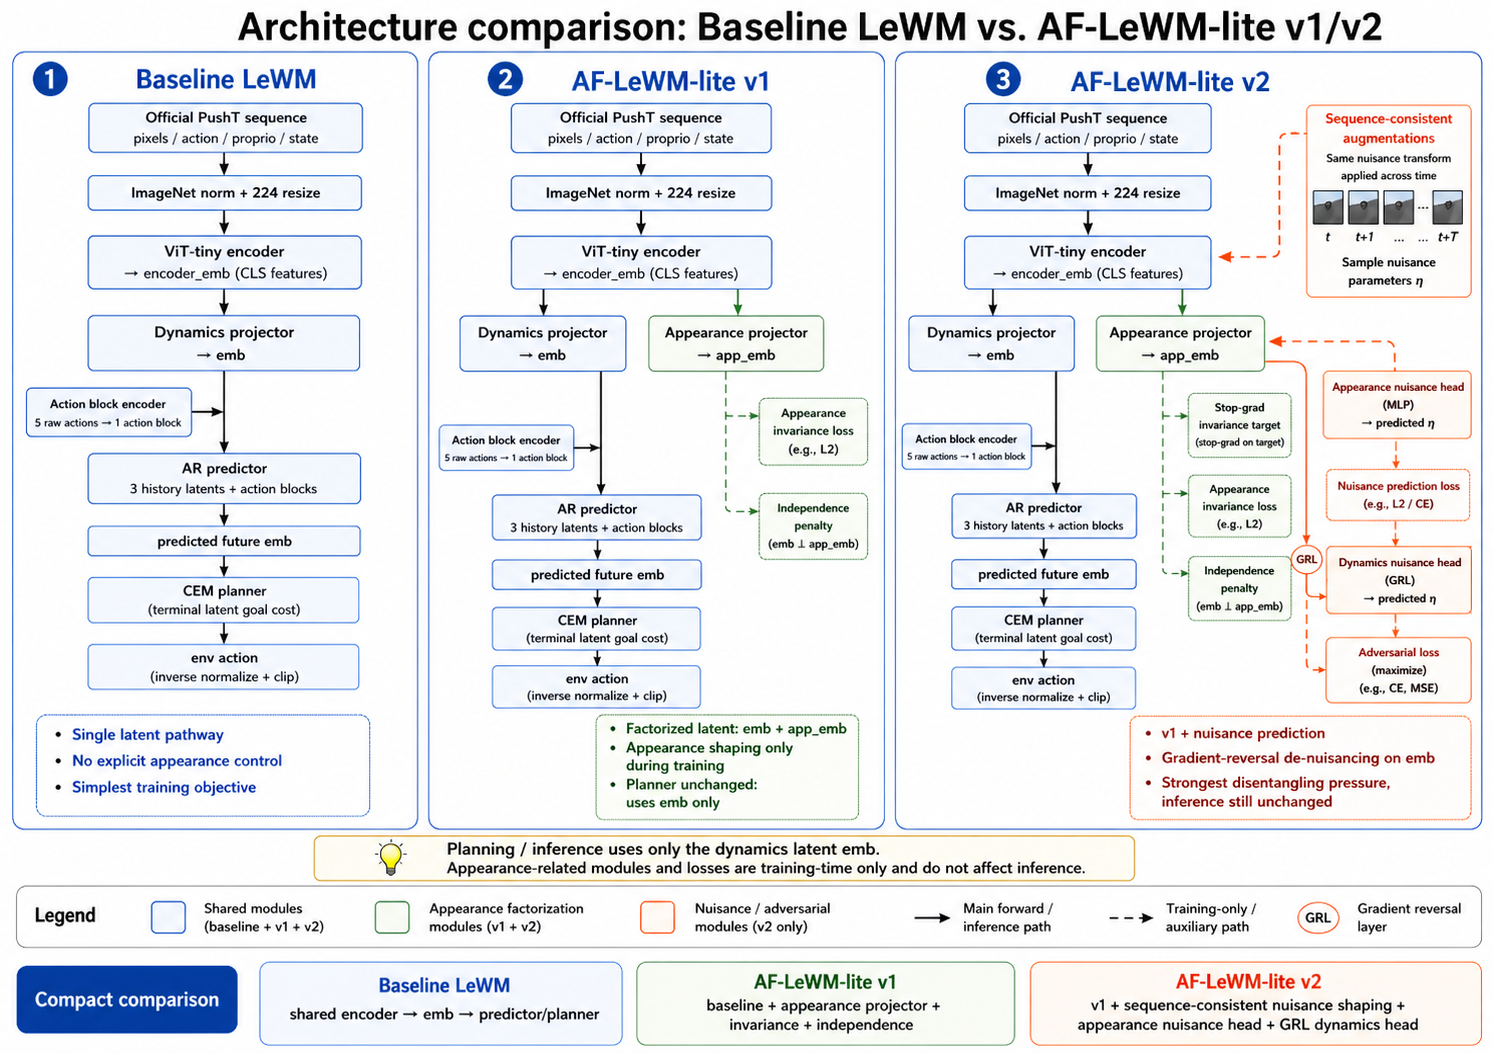
\includegraphics[width=\linewidth]{aflewm_model_pipeline.png}
\caption{Model pipeline. The planner sees only the dynamics branch; appearance heads affect training losses.}
\end{figure}

\section*{Reliable Experiment Protocol}
The rerun uses the official \texttt{pusht\_expert\_train.h5} dataset, an episode-disjoint train/validation split, normalizers fitted only on training episodes, and fresh-run guards that refuse to mix stale checkpoint or metrics artifacts with a new run.

Stage 1 screens every planned structure with train seed 3072, 10 epochs, eval seeds 42 and 43, and 50 PushT episodes per eval seed. Stage 2 scales the selected candidates \texttt{baseline}, \texttt{v1\_current}, and \texttt{v2\_app\_nuisance\_only} with train seeds 3072 and 3073, 50 epochs, eval seeds 42 through 45, and 50 episodes per eval seed. Stage 2 reports epoch-25 and epoch-50 checkpoints, giving 400 evaluation episodes per variant per checkpoint.

\begin{figure}[H]
\centering
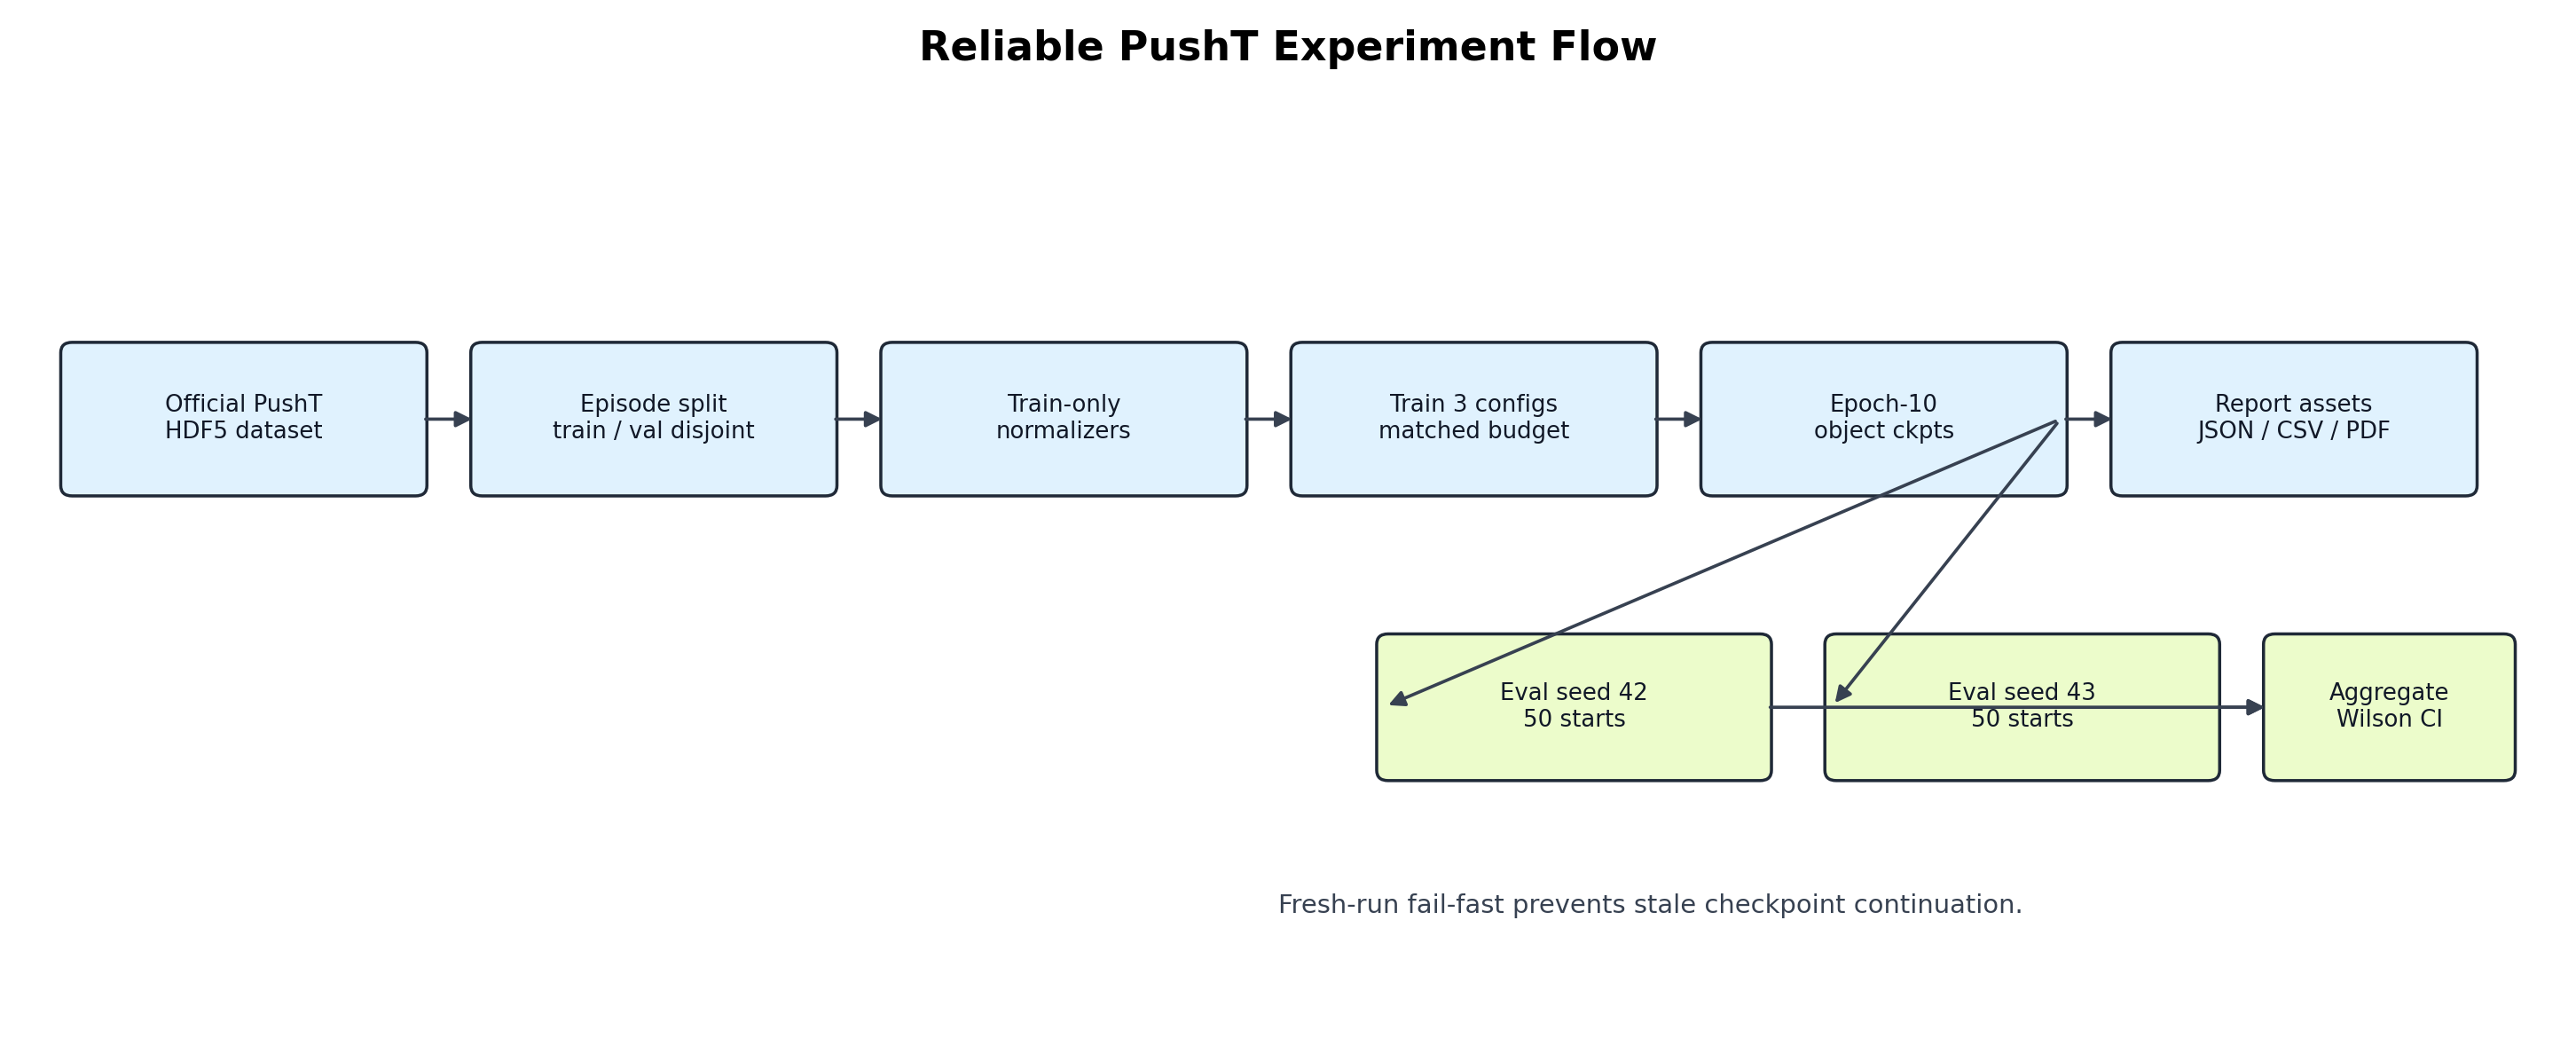
\includegraphics[width=\linewidth]{pusht_experiment_flow.png}
\caption{Experiment flow from official dataset to checked aggregate reports.}
\end{figure}

\section*{Implementation Fixes}
\begin{itemize}[leftmargin=1.2em, itemsep=0.16em, topsep=0.16em]
  \item Training now uses episode-disjoint subsets rather than overlapping clip-level random split.
  \item Evaluation reconstructs the exact training normalizers from the recorded train split metadata.
  \item Fresh reliable runs fail fast when old metrics or checkpoints already exist.
  \item Evaluation reconstructs the raw 15-step history window and compresses it to the model's 3-frame context.
  \item Goal indexing is asserted against the planned raw-step horizon.
  \item PushT goal rendering caches are synchronized after dataset-goal reset before replanning.
  \item Batched CEM evaluates all 50 envs together without expanding pixels or goal images over candidate samples.
  \item CEM candidate actions, elite means, and returned normalized plans are clamped to normalized env action bounds before inverse transform.
  \item Evaluation writes row, episode, start-step, train split, checkpoint, and raw dataset provenance.
\end{itemize}

\begin{figure}[H]
\centering
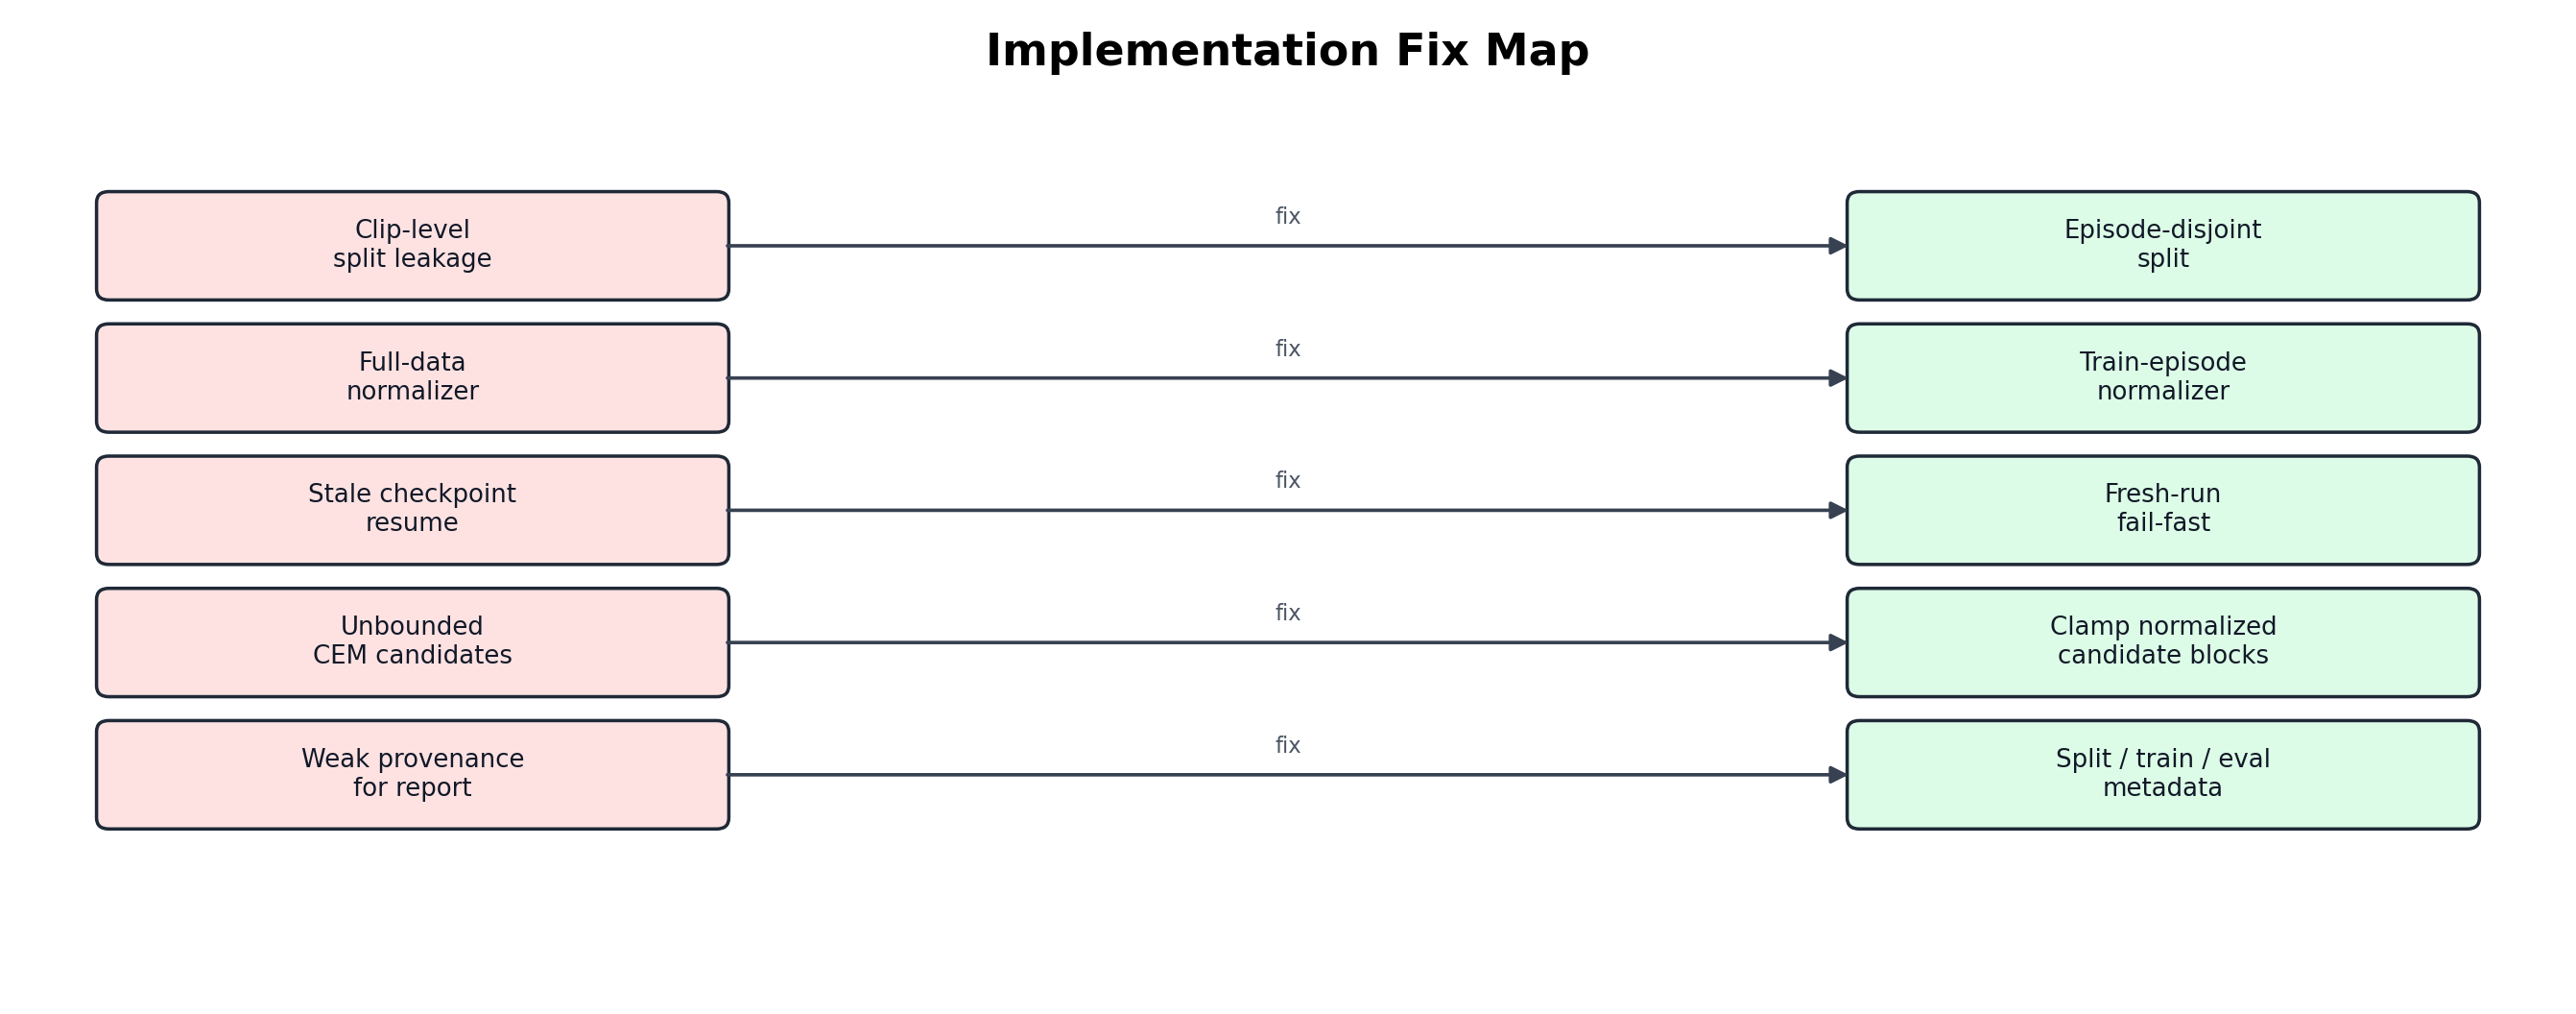
\includegraphics[width=0.95\linewidth]{implementation_fix_map.png}
\caption{Reliability fixes that directly affect whether the experiment tests the intended design.}
\end{figure}

\section*{Results}
\begin{table}[H]
\centering
\scriptsize
\begin{tabular}{llrrrr}
\toprule
Stage 1 variant & Family & Successes & Episodes & Success rate & Delta vs baseline \\
\midrule
\texttt{baseline} & LeWM & 6 & 100 & 6.0\% & 0.0 pp \\
\texttt{v1\_current} & v1 & 10 & 100 & 10.0\% & +4.0 pp \\
\texttt{v1\_inv\_only} & v1 & 2 & 100 & 2.0\% & -4.0 pp \\
\texttt{v1\_indep\_only} & v1 & 5 & 100 & 5.0\% & -1.0 pp \\
\texttt{v1\_seq\_only} & v1 & 5 & 100 & 5.0\% & -1.0 pp \\
\texttt{v1\_seq\_stopgrad} & v1 & 3 & 100 & 3.0\% & -3.0 pp \\
\texttt{v2\_app\_nuisance\_only} & v2 & 8 & 100 & 8.0\% & +2.0 pp \\
\texttt{v2\_weak\_grl} & v2 & 6 & 100 & 6.0\% & 0.0 pp \\
\texttt{v2\_current} & v2 & 5 & 100 & 5.0\% & -1.0 pp \\
\texttt{v2\_grl\_warmup} & v2 & 6 & 100 & 6.0\% & 0.0 pp \\
\bottomrule
\end{tabular}
\caption{Stage 1 structural screen. Two AF candidates beat baseline under the short 100-episode screen.}
\end{table}

\begin{table}[H]
\centering
\small
\begin{tabular}{llrrrr}
\toprule
Checkpoint & Variant & Successes & Episodes & Success rate & Delta vs baseline \\
\midrule
epoch 25 & \texttt{baseline} & 21 & 400 & 5.25\% & 0.00 pp \\
epoch 25 & \texttt{v1\_current} & 19 & 400 & 4.75\% & -0.50 pp \\
epoch 25 & \texttt{v2\_app\_nuisance\_only} & 20 & 400 & 5.00\% & -0.25 pp \\
epoch 50 & \texttt{baseline} & 25 & 400 & 6.25\% & 0.00 pp \\
epoch 50 & \texttt{v1\_current} & 22 & 400 & 5.50\% & -0.75 pp \\
epoch 50 & \texttt{v2\_app\_nuisance\_only} & 20 & 400 & 5.00\% & -1.25 pp \\
\bottomrule
\end{tabular}
\caption{Stage 2 reliability check. The scaled AF candidates trail baseline at both inspected checkpoints.}
\end{table}

\begin{table}[H]
\centering
\scriptsize
\begin{tabular}{llrrrr}
\toprule
Checkpoint & Variant & Train seed & Successes & Episodes & Success rate \\
\midrule
epoch 25 & \texttt{baseline} & 3072 & 11 & 200 & 5.50\% \\
epoch 25 & \texttt{baseline} & 3073 & 10 & 200 & 5.00\% \\
epoch 25 & \texttt{v1\_current} & 3072 & 10 & 200 & 5.00\% \\
epoch 25 & \texttt{v1\_current} & 3073 & 9 & 200 & 4.50\% \\
epoch 25 & \texttt{v2\_app\_nuisance\_only} & 3072 & 8 & 200 & 4.00\% \\
epoch 25 & \texttt{v2\_app\_nuisance\_only} & 3073 & 12 & 200 & 6.00\% \\
epoch 50 & \texttt{baseline} & 3072 & 14 & 200 & 7.00\% \\
epoch 50 & \texttt{baseline} & 3073 & 11 & 200 & 5.50\% \\
epoch 50 & \texttt{v1\_current} & 3072 & 10 & 200 & 5.00\% \\
epoch 50 & \texttt{v1\_current} & 3073 & 12 & 200 & 6.00\% \\
epoch 50 & \texttt{v2\_app\_nuisance\_only} & 3072 & 13 & 200 & 6.50\% \\
epoch 50 & \texttt{v2\_app\_nuisance\_only} & 3073 & 7 & 200 & 3.50\% \\
\bottomrule
\end{tabular}
\caption{Stage 2 per-training-seed detail.}
\end{table}

\section*{Interpretation}
The corrected result should be read conservatively. Stage 1 did not show that all AF variants were weaker than baseline: \texttt{v1\_current} and \texttt{v2\_app\_nuisance\_only} were ahead under the short screen. Stage 2 is the stronger reliability check, and both scaled AF candidates trail baseline there. The current study is useful as a reliability-checked ablation of the AF shaping idea; it does not establish an AF-LeWM-lite PushT improvement.

The main decision is to use baseline as the reliable PushT result for this repo. \texttt{v1\_current} remains valuable as a negative mechanism result because it produces cleaner appearance/dynamics factorization diagnostics, but the cleaner split does not improve planning success under this budget.

\vfill
{\small\color{muted}
Primary machine-readable outputs are the Stage 1 and Stage 2 CSV/JSON summaries under \texttt{report/}.
}

\end{document}
